\documentclass[aspectratio=169,xcolor=dvipsnames]{beamer}
\usetheme{SimplePlus}

% Links
\usepackage{hyperref}
\hypersetup{
    colorlinks=true,
    linkcolor=blue,
    filecolor=magenta,      
    urlcolor=brown,
    linkbordercolor=1 1 1,
    citebordercolor=1 1 1,
    linkbordercolor=1 1 1,
    menubordercolor=1 1 1,
    urlbordercolor=1 1 1,
}

% images
\usepackage{graphicx} 
\usepackage{tikz}

%
\usepackage{booktabs} % Allows the use of \toprule, \midrule and \bottomrule in tables


\title[short title]{\textbf{Credit Card Fraud}} 
\subtitle{Project II Checkpoint I - Artificial Inteligence}
\author[Marcelo  Francisco] {\textbf{Grupo 04\_1A} \\ \begin{tabular}{r l} 
	\email{up201906086@up.pt} & Marcelo Henriques Couto \\
	\email{up201907361@up.pt} & Francisco Pinto de Oliveira \\
\end{tabular}
}

\institute[FEUP] 
{
    Faculdade de Engenharia da Universidade do Porto
}
\date{\today} 



\begin{document}

\begin{frame}
    \tikz [remember picture,overlay]
        \node at
            ([yshift=2.5cm]current page.center) 
            {
\includegraphics[width=.3\textwidth,height=.2\textheight]{images/unnamed.png}};
    \titlepage
\end{frame}


\begin{frame}{Problem Specification}
    \textbf{Credit card fraud} is a crime easily stopable if detected. However, this detection must be quick to occur, as transactions are supposed to be fast. The \textbf{objective} of this project is to \textbf{develop a machine learning model} based on supervised learning classification algorithms able to distinguish, based on some input data, if a given transaction related to a bank account is fraudulent or not. 
        \vspace{0.5em}
        
    In order to come up with the ideal model, we must experiment with at least three different classification algorithms, as well as carry out an \textbf{Exploratory Data Analasys}.

\end{frame}


\begin{frame}{Problem Specification}

    The \href{https://www.kaggle.com/datasets/dhanushnarayananr/credit-card-fraud}{dataset} contains the following data:
    
    \vspace{0.5}
    
    \begin{itemize}
        \item \textbf{Distance from home} - continuous
        \item \textbf{Distance from last transaction} - continuous
        \item \textbf{Ratio to median purchase price: } Ratio of the value of the transaction to the median transaction value - continuous
        \item \textbf{Repeat retailer:} Whether the retailer where the transaction happened had other transactions registered for the same person
        \item \textbf{Used chip:} Transcation via credit card - discrete, binary
        \item \textbf{Used pin number} - discrete, binary
        \item \textbf{Online order} - discrete, binary
        \item \textbf{Fraud} - discrete, binary - \textbf{label}
    \end{itemize}
    We considered that all distances are expressed in kilometers.
\end{frame}
\begin{frame}{Related Work}
    \textbf{Code}
    \begin{itemize}
        \item \href{https://imbalanced-learn.org/stable/}{Imbalanced Learn} - over sampling and undersampling tools
        \item \href{https://scikit-learn.org/}{Scikit Learn} - machine learning algorithms
    \end{itemize}
    
    \vspace{0.5em}
    
    \textbf{Websites}
    \begin{itemize}
        \item \href{https://machinelearningmastery.com/what-is-imbalanced-classification/}{https://machinelearningmastery.com/what-is-imbalanced-classification/}
        \item \href{https://developers.google.com/machine-learning/data-prep/construct/sampling-splitting/imbalanced-data}{https://developers.google.com/machine-learning/data-prep/construct/sampling-splitting/imbalanced-data}
    \end{itemize}
        \vspace{0.5em}
    
    \textbf{Articles}
    \begin{itemize}
        \item Bekkar, M., Djemaa, H. K., & Alitouche, T. A. (2013). Evaluation measures for models assessment over imbalanced data sets. J Inf Eng Appl, 3(10).
        \item Tharwat, A. (2021), "Classification assessment methods", Applied Computing and Informatics, Vol. 17 No. 1, pp. 168-192. 
    \end{itemize}
\end{frame}
\begin{frame}{Tools and Algorithms}

    \textbf{Tools}
    \vspace{0.5em}
    
    We will use \textbf{Python} as programming language, programming in a \textbf{Jupyter Notebook} environment. For machine learning algorithms, we will resource to \textbf{Scikit-Learn} and \textbf{Imbalanced Learn} libraries, as well as \textbf{Pandas} to read and handle the data and \textbf{Seaborn and Matplotlib} to visualize it.

    \vspace{1em}
    
    \textbf{Algorithms}
    \vspace{0.5em}
    
    Because our dataset is imbalanced, we plan to explore \textbf{Synthetic Minority Oversampling} and \textbf{Undersampling} techniques to handle this issue.

    \vspace{0.5em}
    
    For the classification we plan on using \textbf{Logistic Regression}, \textbf{Random Forest}, \textbf{Decision Trees}, \textbf{Neural Networks} and possibly others.

\end{frame}




\begin{frame}{Implementation Already Carried Out}
    \textbf{Language: } Python - Anaconda \\
    \vspace{0.5em}
    \textbf{Environment: } Visual Studio Code using JupyterNotebooks \\
    \vspace{0.5em}
    \textbf{Data Structures:} 
    The dataset is represented as a
    \href{https://pandas.pydata.org/docs/reference/api/pandas.DataFrame.html}{pandas.DataFrame}
    \vspace{0.5em}
    \textbf{Data Preprocessing} and \textbf{Exploratory Data Analysis}:
    \begin{itemize}
        \item Analysis of dataset's validity and integrity
        \item Analysis of dataset balance
        \item Analysis of outliers, missing values and other errors
        \item Analysis of correlations between the multiple variables
    \end{itemize}
        \vspace{0.5em}
    \textbf{Model Training}
    \begin{itemize}
        \item Logistic Regression with cross validation using Area Under ROC Curve as evaluation measure
    \end{itemize}
\end{frame}

\begin{frame}{Data Pre-Processing}

    \begin{minipage}{0.5\textwidth}
          Our data set presented to be ready to use as:
        \begin{itemize}
            \item There were no missing values
            \item There were no apparent measurement errors
            \item There were many outliers but they did not represent any errors and were, in all likelihood, the exact object of our analysis
        \end{itemize}
    \end{minipage}%
    \begin{minipage}{0.5\textwidth}
        \begin{figure}
            \centering
            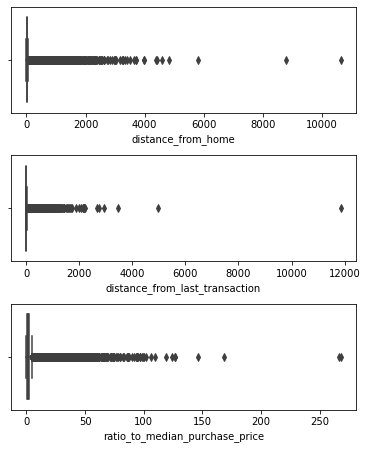
\includegraphics[width=0.65\textwidth]{images/boxplots.png}
            \caption{Boxplots}
            \label{fig:my_label}
        \end{figure}
    \end{minipage}

\end{frame}

\begin{frame}{Exploratory Data Analysis}

    \begin{minipage}{0.5\textwidth}
        Performing an \textbf{Exploratory Data Analysis} we concluded that:
        \begin{itemize}
            \item As previously mentioned, our data set was moderately imbalanced (classification label is binary and 8.7\% of the entries represent fraudulent transactions).
            \item Many of the features had little relation with the label feature, as their values did not vary much between the two label classes and their correlation was very low. 
        \end{itemize}
    \end{minipage}%
    \begin{minipage}{0.5\textwidth}
        \begin{figure}
            \centering
            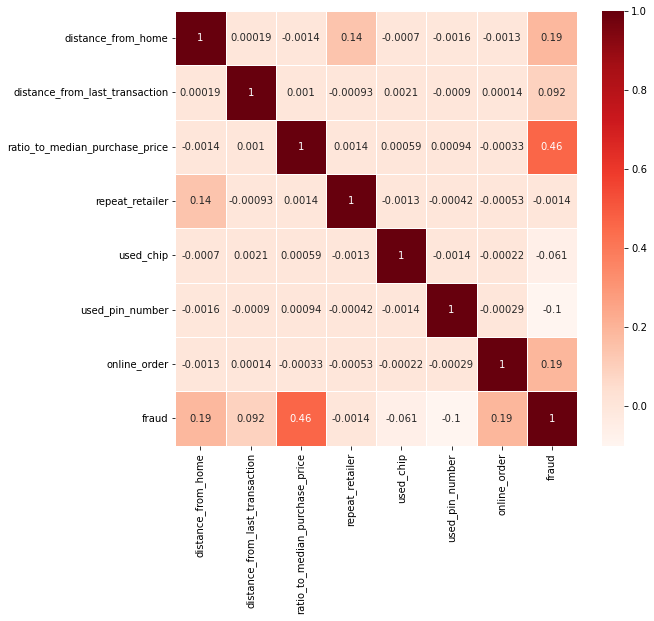
\includegraphics[width=0.85\textwidth]{images/output.png}
            \caption{Correlation Matrix}
            \label{fig:my_label}
        \end{figure}
    \end{minipage}

    
    
    
\end{frame}


\begin{frame}{Machine Learning Models}

    The algorithms we chose to train our models were:
    \begin{itemize}
        \item \textbf{Logistic Regression(LR):} Good with binary data, easy and simple to understand
        \item \textbf{Decision Tree(DT):} Decently robust to imbalanced datasets and irrelevant features
        \item \textbf{K Nearest Neighbours(KNN):} Overall simple
        \item \textbf{Random Forest(RF):} Handles imbalanced datasets well and is impervious to overfitting
        \item \textbf{Multilayer Perceptron(MLP):} Very powerful all arround
    \end{itemize}
    
    \textbf{Notes:}
    \begin{itemize}
        \item KNN was only tested with smaller data sets due to elevated training and testing times (lack of processing power)
        \item Logistic Regression was tested with a dataset where a column had been removed, in an attempt to fight the algorithm's sensitivity to irrelevant features
        \item All algorithms but MLP were tested with Grid Search with portions of the data set, in order to find the best parameters for the final model
    \end{itemize}
\end{frame}

\begin{frame}{Model Evaluation and Comparison}
    \begin{center}
        \scalebox{0.65}{
            \begin{table}[]
        \begin{tabular}{|l|l|l|l|l|l|l|l|}
        \hline
        \textbf{Model}             & \textbf{Time to train (s)} & \textbf{Time to test (s)} & \textbf{Recall}   & \textbf{Roc Auc}  & \textbf{Precision} & \textbf{Accuracy} & \textbf{Balanced Accuracy} \\ \hline
        lr\_control\_full & 19.497249         & 0.005409         & 0.599163 & 0.796077 & 0.890613  & 0.95874  & 0.796077          \\ \hline
        lr\_smoted\_full  & 55.498035          & 0.015769         & 0.980637 & 0.943067 & 0.497086  & 0.912032 & 0.943067          \\ \hline
        lr\_weight\_full  & 120.202866        & 0.016395         & 0.97291  & 0.94429  & 0.523563  & 0.920648 & 0.94429           \\ \hline
        dt\_control\_full & 12.073779         & 0.008223         & 0.999908 & 0.999952 & 0.999954  & 0.999988 & 0.999952          \\ \hline
        dt\_smoted\_full  & 26.15653          & 0.016174         & 0.999862 & 0.999922 & 0.999816  & 0.999972 & 0.999922          \\ \hline
        dt\_weight\_full  & 6.897408          & 0.015349         & 0.999908 & 0.999952 & 0.999954  & 0.999988 & 0.999952          \\ \hline
        mlp\_normal\_full & 960.845785        & 0.208947         & 0.892052 & 0.945036 & 0.977226  & 0.988804 & 0.945036          \\ \hline
        rf\_control\_full & 361.549095        & 1.325936         & 0.999908 & 0.999954 & 1         & 0.999992 & 0.999954          \\ \hline
        rf\_smoted\_full  & 132.806744        & 0.117373         & 0.999908 & 0.99995  & 0.999908  & 0.999984 & 0.99995           \\ \hline
        rf\_weight\_full  & 303.098518        & 0.771723         & 0.999908 & 0.999952 & 0.999954  & 0.999988 & 0.999952          \\ \hline
        knn\_control\_10p & 19.848561         & 47.906985        & 0.828354 & 0.904025 & 0.79605   & 0.966481 & 0.904025          \\ \hline
        knn\_smoted\_10p  & 233.760107        & 181.564677       & 0.989553 & 0.993826 & 0.980322  & 0.997353 & 0.993826          \\ \hline
        knn\_none\_10p    & 119.013859        & 121.487901       & 0.983827 & 0.991484 & 0.990951  & 0.997803 & 0.991484          \\ \hline
        \end{tabular}
        \end{table}
                }
    \end{center}
    
    \textbf{Note:} \textbf{control} are models trained with default parameters, \textbf{weight} are models trained on normal data sets but best parameters in grid search (focusing fixing the imbalance with class weights), \textbf{smote} are models trained with best parameters from grid search and using \textbf{SMOTE} in training data set, \textbf{none} is the same as weight but without class weights (for parameter details, check notebook)
\end{frame}

\begin{frame}{Model Evaluation and Comparison}


\begin{figure}
    \centering
    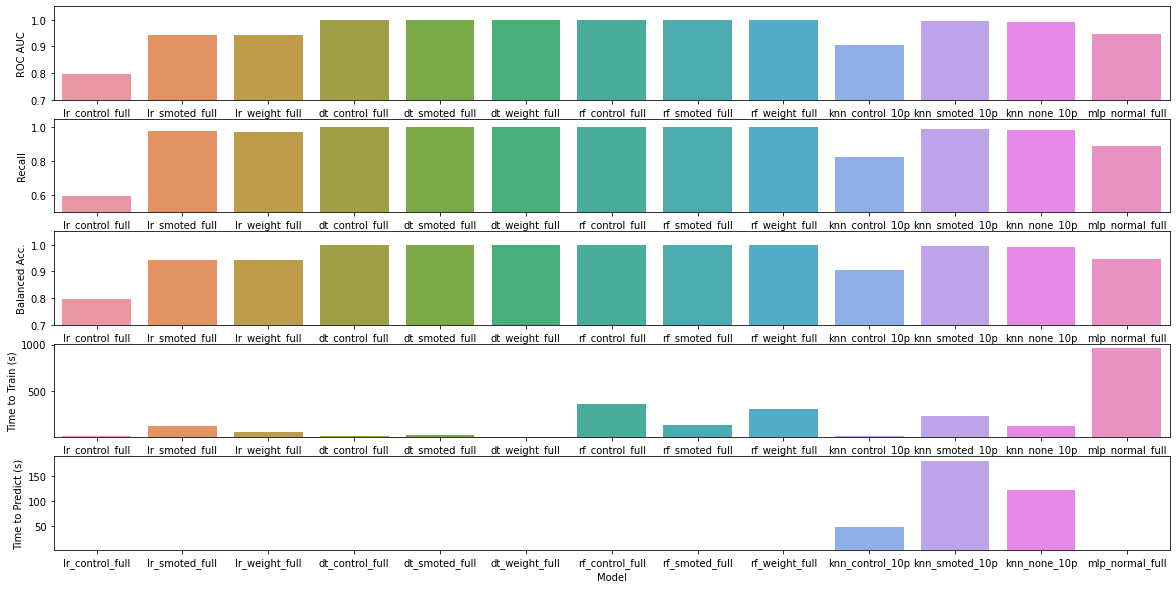
\includegraphics[width=.85\textwidth]{images/plots.png}
    \caption{Model Scores and Times}
    \label{fig:my_label}
\end{figure}
\end{frame}
\begin{frame}{Conclusions}
    
    From the graphs and table we are able to conclude that:
    \begin{itemize}
        \item The best models were the ones based in Random Forest and Decision Tree algorithms, which goes accordingly to their resistance against imbalance. Random Forest did not present much advantage as the Decision Tree models already featured perfect scores and clearly did not suffer from overfitting
        \item The worse models were the ones based in Logistic Regression algorithms, most likely because of their sensitivity to imbalance and overall lack of robustness
        \item K Nearest Neighbours models were way too slow to be a viable option, so much so that we only trained and tested with 10\% of the data set
        \item Multi-layer Perceptron based models were not worth the complexity, as their results were not their great and the training time was big
        \item SMOTE and class weights had a decent impact in LR, yet they did not show mutch effects on the other algorithms
    \end{itemize}

\end{frame}

\end{document}